\documentclass{article}
\usepackage[utf8]{inputenc}
\usepackage{graphicx}

\title{Rapport synthèse projet}
\author{Manon Lécubin, Aurélie Demure, Pierre Auguste, Nicolas Fernandez}
\date{October 2022}

\begin{document}

\maketitle

\section{Charte Projet}

\subsection{Contexte}

Aujourd'hui, les circuits courts sont les alternatives les plus intéressantes face au défi qu'est devenu la gestion de l'alimentation et de l'eau. De nombreuses solutions sont apparues pour faire face à ce défi. On peut retrouver les jardins partagés, les micro-fermes mais également le partage de ressources produites au sein de jardins privés. 

Ces applications sont principalement utilisées par les propriétaires de jardin privés. Chacune d'entre elles permet de répondre à sa manière à la problématique du surplus de production dans ces jardins ainsi que leur gestion.

Le cahier des charges permet d'identifier de manière immédiate les principaux besoins et fonctions auxquels l'application doit répondre. Il s'agit notamment de permettre de mettre en relation des propriétaires de jardins privés, de permettre de gérer le surplus de production mais également de permettre une meilleure gestion de la récolte afin d'éviter les pertes initiales.


\subsection{Finalités et importance du projet: Business Case}

Ce projet est aujourd'hui essentiel afin de répondre aux problématiques actuelles concernant la gestion de l'alimentation en circuits courts. De plus, la nature même du projet et ses coûts extrêmements limités réduisent la néceesité d'un retour sur investissement, permettant ainsi un départ peu risqué. L'application visant à proposer un service sans recherche de bénéfices, l'estimation de ces derniers est inutile.

De manière prévisionnelle, on peut estimer que l'application permettra de mettre en relation de nombreux propriétaires de jardins privés au sein de communes principalement en zone rurale. Sa gestion des récoltes participera à une nouvelle manière de partager des surplus de fruits non consommés, une innovation qui permettra une ouverture plus grande que la plupart des projets existants.

\vspace{4mm}

Les parties prenantes relatives au projets sont: l'équipe projet, composée de quatre membres, les enseignants encadrants, ainsi que les potentiels utilisateurs de l'application.

Le périmètre du projet s'étend sur tout le territoire français, mais la nature même de son fonctionnement favorise une utilisation dans des zones rurales où le nombre de jardins privés est bien plus important.
A cette limite géographique s'ajoutent de nombreux prérequis à obtenir: obtention des compétences nécessaires au développement d'une application web et de la création d'algorithme, être dans un cadre légal quant à la possibilité de venir récolter les fruits chez une autre personne.

\vspace{4mm}
 
Cette analyse du Business Case permet de proposer une matrice SWOT identifiant les forces, faiblesses, opportunités ainsi que menaces du projet.

\vspace{2mm}             
  
\begin{centering}
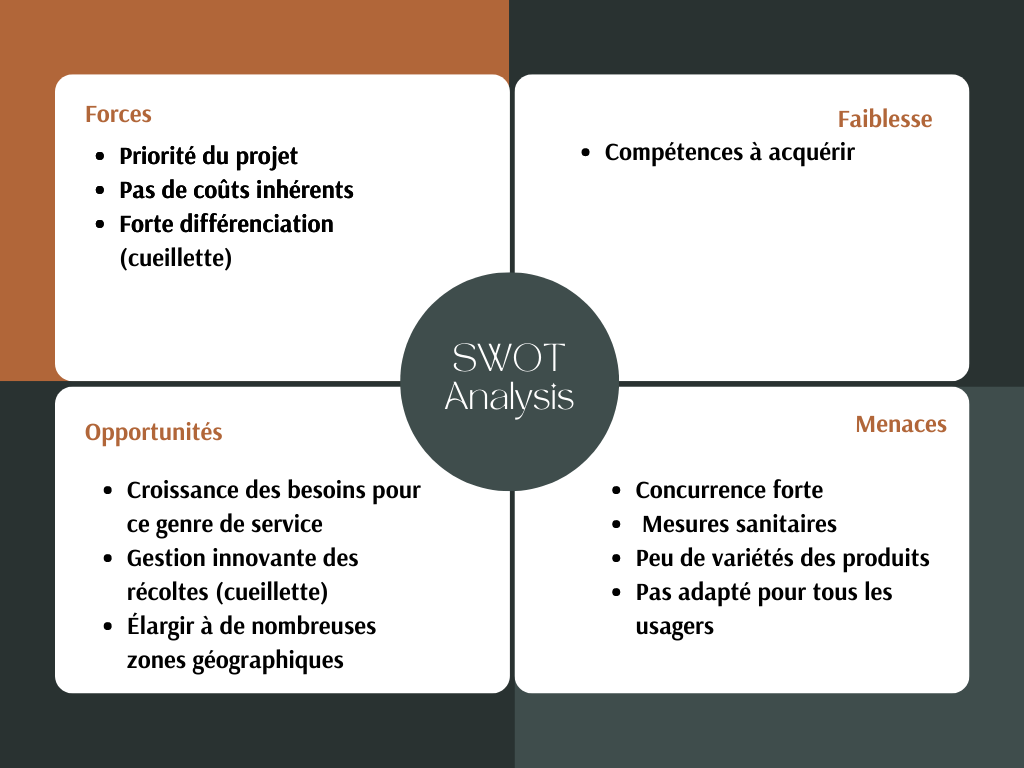
\includegraphics[width = 12cm, height = 9 cm]{SWOTF.png}
\end{centering}

\maketitle
\subsection{Objectifs et résultats opérationnels}

Ces applications connaissent un franc succès aujourd'hui, de par la nécessité de faire face au défi du gaspillage alimentaire, ainsi que par le développement des circuits courts. L'innovation ici proposée, concernant la participation à la récolte même des fruits, permet de s'attaquer à l'une des principales causes de perte de ces derniers. Ces différents éléments sont des indicateurs de la possibilité de succès de ce projet.

\subsection{Ressources}
Les moyens à mobiliser sont :
PC personnels et/ou de l'école, postgress4SQL, python3 


\subsection{Jalons}
\begin{center}
\begin{tabular}{|p{3cm}|p{5cm}|p{2cm}|} 
  \hline
  Jalon & Description & Date \\
  \hline
  Etape 1 : Exigences opérationnelles & Validation de l'idée lors de la soutenance & 22/10/22 \\
  \hline
  Etape 2 : Création de la base de données & Création de la base de données relative aux fruits et légumes disponibles &  \\
  \hline
  Etape 3 : Réalisation de l'interface & Réalisation de l'interface utilisateur & \\
  \hline
  Etape 4 : Réalisation messagerie & 
  Réalisation d'un système de contact entre les utilsateurs (messagerie) pour obtenir plus d'informations sur un produit en vente ou les conditions d'accueil pour une cueillette & \\
  \hline
  Etape 5 : Ajout d'une carte & Ajout d'une carte permettant de repérer où se situent les fruits et légumes & \\
  \hline
  Etape 6 : Ajout de restrictions sur la carte & Ajouter des rayons sur la carte par rapport à la localisation du client, qui augmentent au cours du temps & \\
  \hline
  Etape 7 : Ajout d'une fonctionnalité pour les dons & Ajouter une fonction qui permet au client de donner ses produits dans les derniers jours de consommation possibles du produit & \\ 
  \hline
\end{tabular}
\end{center}


\end{document}
